\problemname{Clock Pictures}

You have two pictures of an unusual kind of clock. The clock has $n$ hands, each having the same length and no kind of marking whatsoever. Also, the numbers on the clock are so faded that you can't even tell anymore what direction is up in the picture. So the only thing that you see on the pictures, are $n$ shades of the $n$ hands, and nothing else.

You'd like to know if both images might have been taken at exactly the same
time of the day, possibly with the camera rotated at different angles.

\section*{Task}

Given the description of the two images, determine whether it is possible that these two pictures could be showing the same clock displaying the same time.

\section*{Input}

The first line contains a single integer $n$ ($2 \leq n \leq 200\, 000$), the number of hands on the clock.

Each of the next two lines contains $n$ integers $a_i$ ($0 \leq a_i <
360\, 000$), representing the angles of the hands of the clock on one
of the images, in thousandths of a degree. The first line represents
the position of the hands on the first image, whereas the second line
corresponds to the second image. The number $a_i$ denotes the angle
between the recorded position of some hand and the upward direction in
the image, measured clockwise. Angles of the same clock are distinct
and are not given in any specific order.

\section*{Output}

Output one line containing one word: \verb+possible+ if the clocks could be showing the same time, \verb+impossible+ otherwise.

\begin{figure}[h]
  \centering
  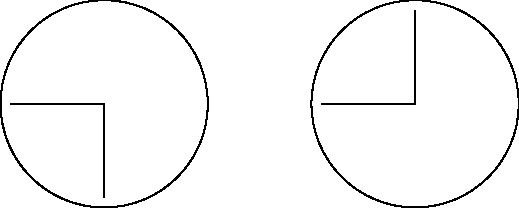
\includegraphics[width=0.45\textwidth]{sample2}
  \caption{Sample input 2}
  \label{fig:sample2}
\end{figure}
